\documentclass[]{onethree}

% single-column: \documentclass[]{onethree}
% twocolumn: \documentclass[twocolumn]{onethree}

\usepackage[toc,page,header]{appendix}
\usepackage{minitoc}
\usepackage{amsmath,amssymb}
\usepackage{bm}
\usepackage{wrapfig}
\usepackage{enumitem}

% Placeholder figure used throughout the template. Replace the box content with
% \includegraphics when adding final paper figures.
\newcommand{\templatefigure}[2][0.95\linewidth]{%
  \fbox{%
    \begin{minipage}[c][0.28\linewidth][c]{#1}
      \centering\sffamily\small
      #2\\[0.6em]
      Replace with final figure or table artwork.
    \end{minipage}%
  }%
}

\title{Paper Title: Concise Subtitle Describing the Main Contribution}

\author[1]{First Author}
\author[1,2]{Second Author}
\author[2]{Third Author}

\affiliation[1]{Institution One}
\affiliation[2]{Institution Two}

\abstract{
This template supports arXiv-style papers with a polished title block, resource links, figures, references, and appendix material.
Replace this text with a concise summary of the problem, method, contribution, and main findings.
Use the remaining sentences to describe the main technical idea, the evaluation setting, and the most important result or takeaway.
The final version may also point readers to released project pages, code repositories, models, datasets, demos, or supplementary materials.
\vspace{-0.1cm}
}

\checkdata[Resources]{
  \href{https://choucisan.github.io}{\raisebox{-1ex}{
\includegraphics[height=4.2ex]{assets/internet-icon.pdf}}~Project Page}\hspace{2em}
  \href{https://github.com/choucisan}{\raisebox{-1ex}{
\includegraphics[height=4.2ex]{assets/github-logo.pdf}}~Code}\hspace{2em}
  \href{https://huggingface.co/choucsan}{\raisebox{-1ex}{
\includegraphics[height=4.2ex]{assets/hf-logo.pdf}}~Hugging Face}
}

\begin{document}
\maketitle
\vspace{-1.1cm}

\begin{figure}[!htbp]
  \centering
  \includegraphics[width=0.98\linewidth]{pngs/image.png}
  \caption{\textbf{Paper overview.} Replace this placeholder image with the main teaser, pipeline summary, or key result figure.}
  \label{fig:teaser}
\end{figure}

\newpage

\tableofcontents
\newpage

% If the paper should not include a table of contents, comment out the three
% lines above. Keep the title page and contents on separate pages.

\section{Introduction}

Introduce the research problem and explain why it matters.
This opening paragraph should define the application setting, the current limitations of prior work, and the practical or scientific motivation for the paper.
Use concrete language, but avoid implementation details that belong in later sections.

Summarize the central gap addressed by the paper.
For example, the gap may involve quality, efficiency, robustness, scalability, interpretability, data availability, or deployment constraints.
Frame the gap in a way that prepares the reader for the proposed method.

Briefly describe the proposed approach.
This paragraph should give the reader a high-level mental model of the system, algorithm, dataset, or analysis before the technical sections begin.
Refer to the main overview figure when appropriate, such as Figure~\ref{fig:teaser}.

The main contributions can be listed as follows:
\begin{itemize}
    \item \textbf{Contribution One.} Describe the first technical or empirical contribution in one or two sentences.
    \item \textbf{Contribution Two.} Describe the second contribution, emphasizing what is new or useful.
    \item \textbf{Contribution Three.} Describe the validation, dataset, benchmark, application, or analysis contribution.
\end{itemize}

Close the introduction with a short summary of the evidence supporting the paper's claims.
Mention the evaluation setting, important metrics, and broad conclusions without including final numeric results until they are ready for release.

\newpage

\section{Method}

This section should present the proposed method at a level that allows readers to understand and reproduce the core idea.
Start with a short overview of the full pipeline, then introduce each component in the order it is used.

\subsection{Problem Formulation}

Define the inputs, outputs, assumptions, and notation.
For example, let $x$ denote the input, $y$ denote the target output, and $f_\theta$ denote the model or algorithm being optimized.
Clarify whether the setting is supervised, self-supervised, generative, interactive, or analytical.

\subsection{System Overview}

\begin{figure}[t]
    \centering
    \includegraphics[width=0.95\linewidth]{pngs/image1.png}
    \caption{\textbf{Method overview.} Replace this placeholder with a diagram of the proposed pipeline, including inputs, major modules, and outputs.}
    \label{fig:method_overview}
\end{figure}

Describe the major components shown in Figure~\ref{fig:method_overview}.
Keep this subsection conceptual; details such as architecture, losses, and implementation choices can be moved to later subsections.

\subsection{Core Module}

Explain the main technical component.
State what problem it solves, what information it consumes, and what representation or prediction it produces.
If the method uses a neural architecture, describe the backbone, conditioning signals, and output heads.
If the method is not neural, describe the algorithmic stages and decision rules.

\subsection{Objective}

Provide the training or optimization objective.
Use equations for important losses and define each term immediately after it appears:
\begin{equation}
    \mathcal{L} = \lambda_1 \mathcal{L}_{\mathrm{main}} + \lambda_2 \mathcal{L}_{\mathrm{reg}}.
\end{equation}
Here, $\mathcal{L}_{\mathrm{main}}$ is the primary task loss and $\mathcal{L}_{\mathrm{reg}}$ is an optional regularization term.

\subsection{Implementation Details}

Summarize implementation choices that are needed for reproducibility, including model size, optimizer, learning rate schedule, batch size, hardware, and relevant preprocessing.
Move lengthy details to the appendix when they interrupt the main narrative.

\section{Data}
\label{sec:data}

\begin{figure*}[t]
  \centering
  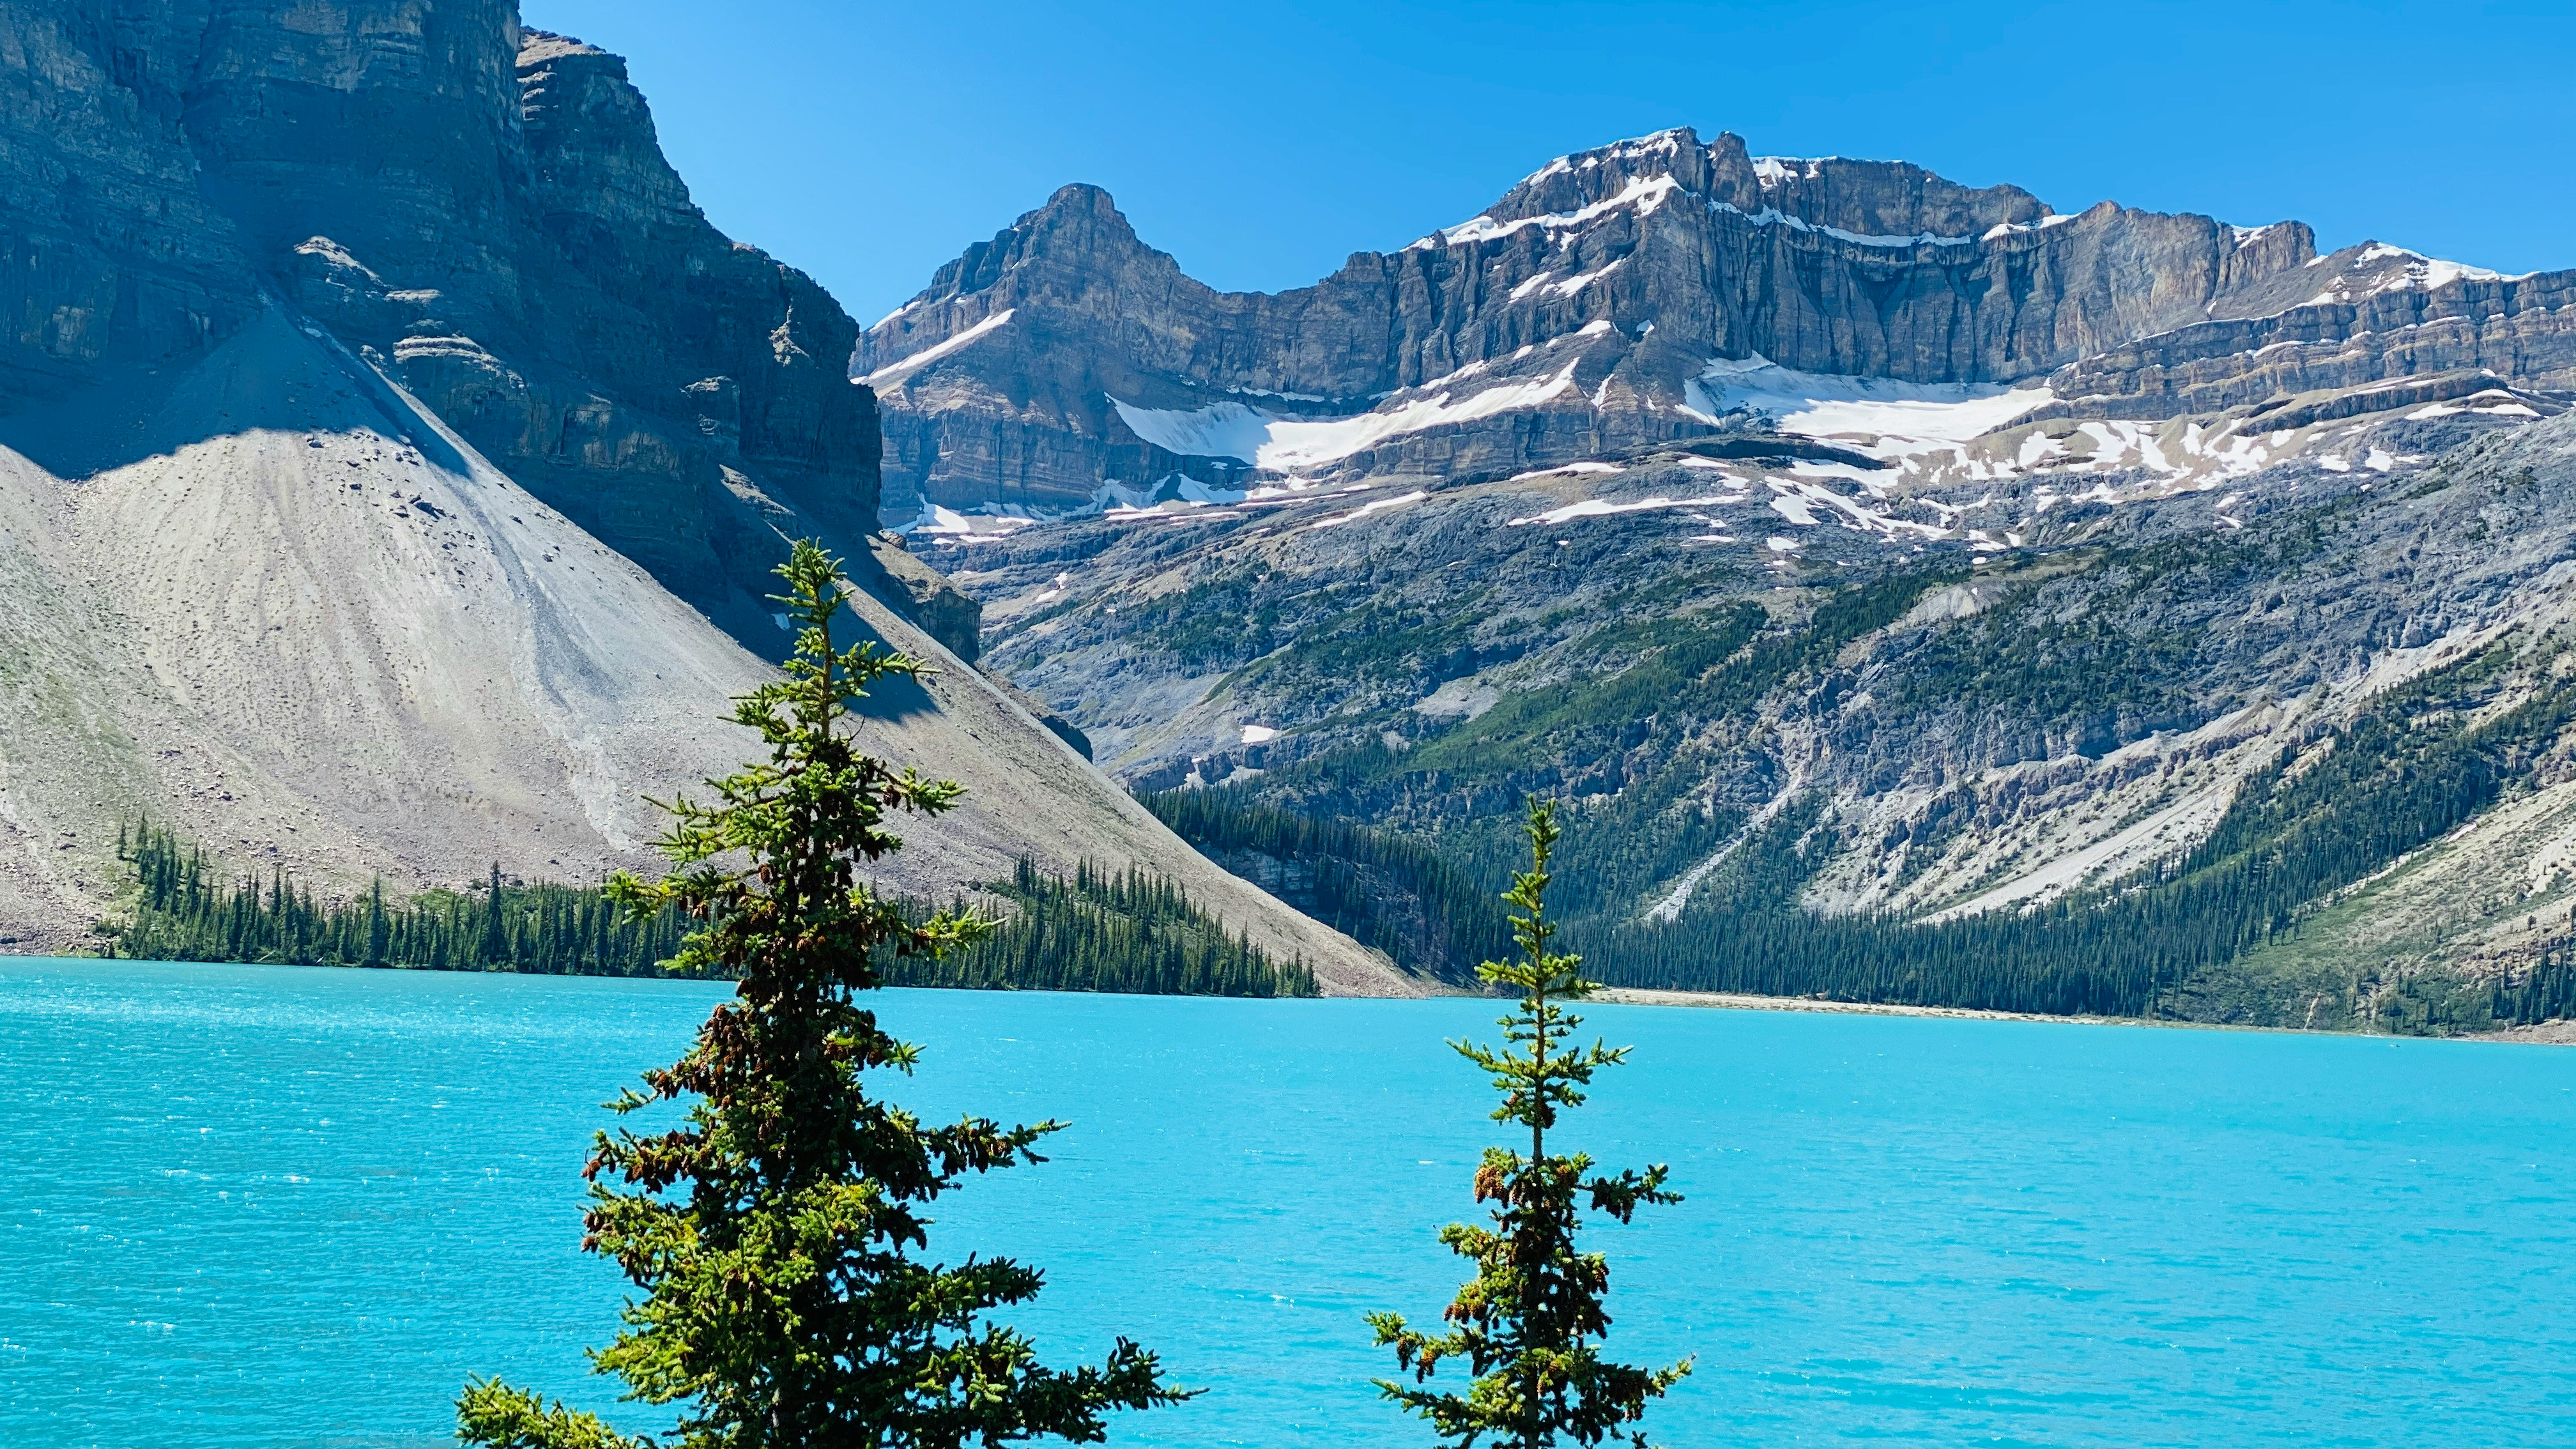
\includegraphics[width=0.92\linewidth]{pngs/image2.png}
  \caption{\textbf{Data pipeline.} Replace this placeholder with a dataset construction, preprocessing, or annotation workflow.}
  \label{fig:data_pipeline}
\end{figure*}

Describe the data sources, collection protocol, filtering criteria, annotation process, and dataset splits.
Include enough detail for readers to understand the scope and limitations of the data without exposing private or unreleased information.

\textbf{Collection.}
Explain where the data comes from and what inclusion criteria were applied.
If applicable, report the number of samples, domains, classes, annotators, or acquisition devices.

\textbf{Preprocessing.}
Describe cleaning, normalization, deduplication, quality control, and format conversion.
Reference Figure~\ref{fig:data_pipeline} if the pipeline is shown visually.

\textbf{Splits and Usage.}
State how training, validation, and test splits are constructed.
Mention measures taken to prevent leakage between splits.

\textbf{Ethics and Licensing.}
Summarize consent, privacy, licensing, and safety considerations when they apply.
For public datasets, cite the original sources, such as a placeholder reference~\cite{sample_reference}.

\section{Training}

\subsection{Training Setup}

Describe the training recipe used for the main model or algorithm.
Include the optimizer, learning rate schedule, batch size, number of steps or epochs, hardware, precision, and checkpoint selection policy.

\subsection{Curriculum or Stages}

If the method uses multiple training stages, describe them in chronological order:
\begin{itemize}
    \item \textbf{Stage 1.} State the purpose of the first stage and the data used.
    \item \textbf{Stage 2.} State how the second stage changes the objective, data, resolution, or supervision.
    \item \textbf{Final Tuning.} State any final adaptation, calibration, or selection step.
\end{itemize}

\subsection{Ablations During Development}

Briefly describe the design choices that were tested while developing the method.
Detailed ablation results can be reported in Section~\ref{sec:evaluation} or in the appendix.

\section{Inference and Deployment}

\subsection{Inference Pipeline}

Describe how a trained model or finalized method is used at test time.
State the required inputs, preprocessing steps, decoding or post-processing steps, and expected outputs.
If the inference procedure differs from training, explain the difference clearly.

\subsection{Efficiency}

Report runtime, memory usage, model size, or computational complexity when relevant.
Use a table if several variants are compared.
Avoid hard-coded claims until the final benchmark numbers have been verified.

\subsection{Practical Considerations}

Mention constraints that matter for real use, such as input resolution, supported formats, batching behavior, failure cases, or compatibility with downstream tools.

\section{Experiments}
\label{sec:evaluation}

This section should substantiate the paper's main claims.
Start by naming the evaluation tasks, datasets, metrics, and baselines.

\begin{figure*}[!h]
  \centering
  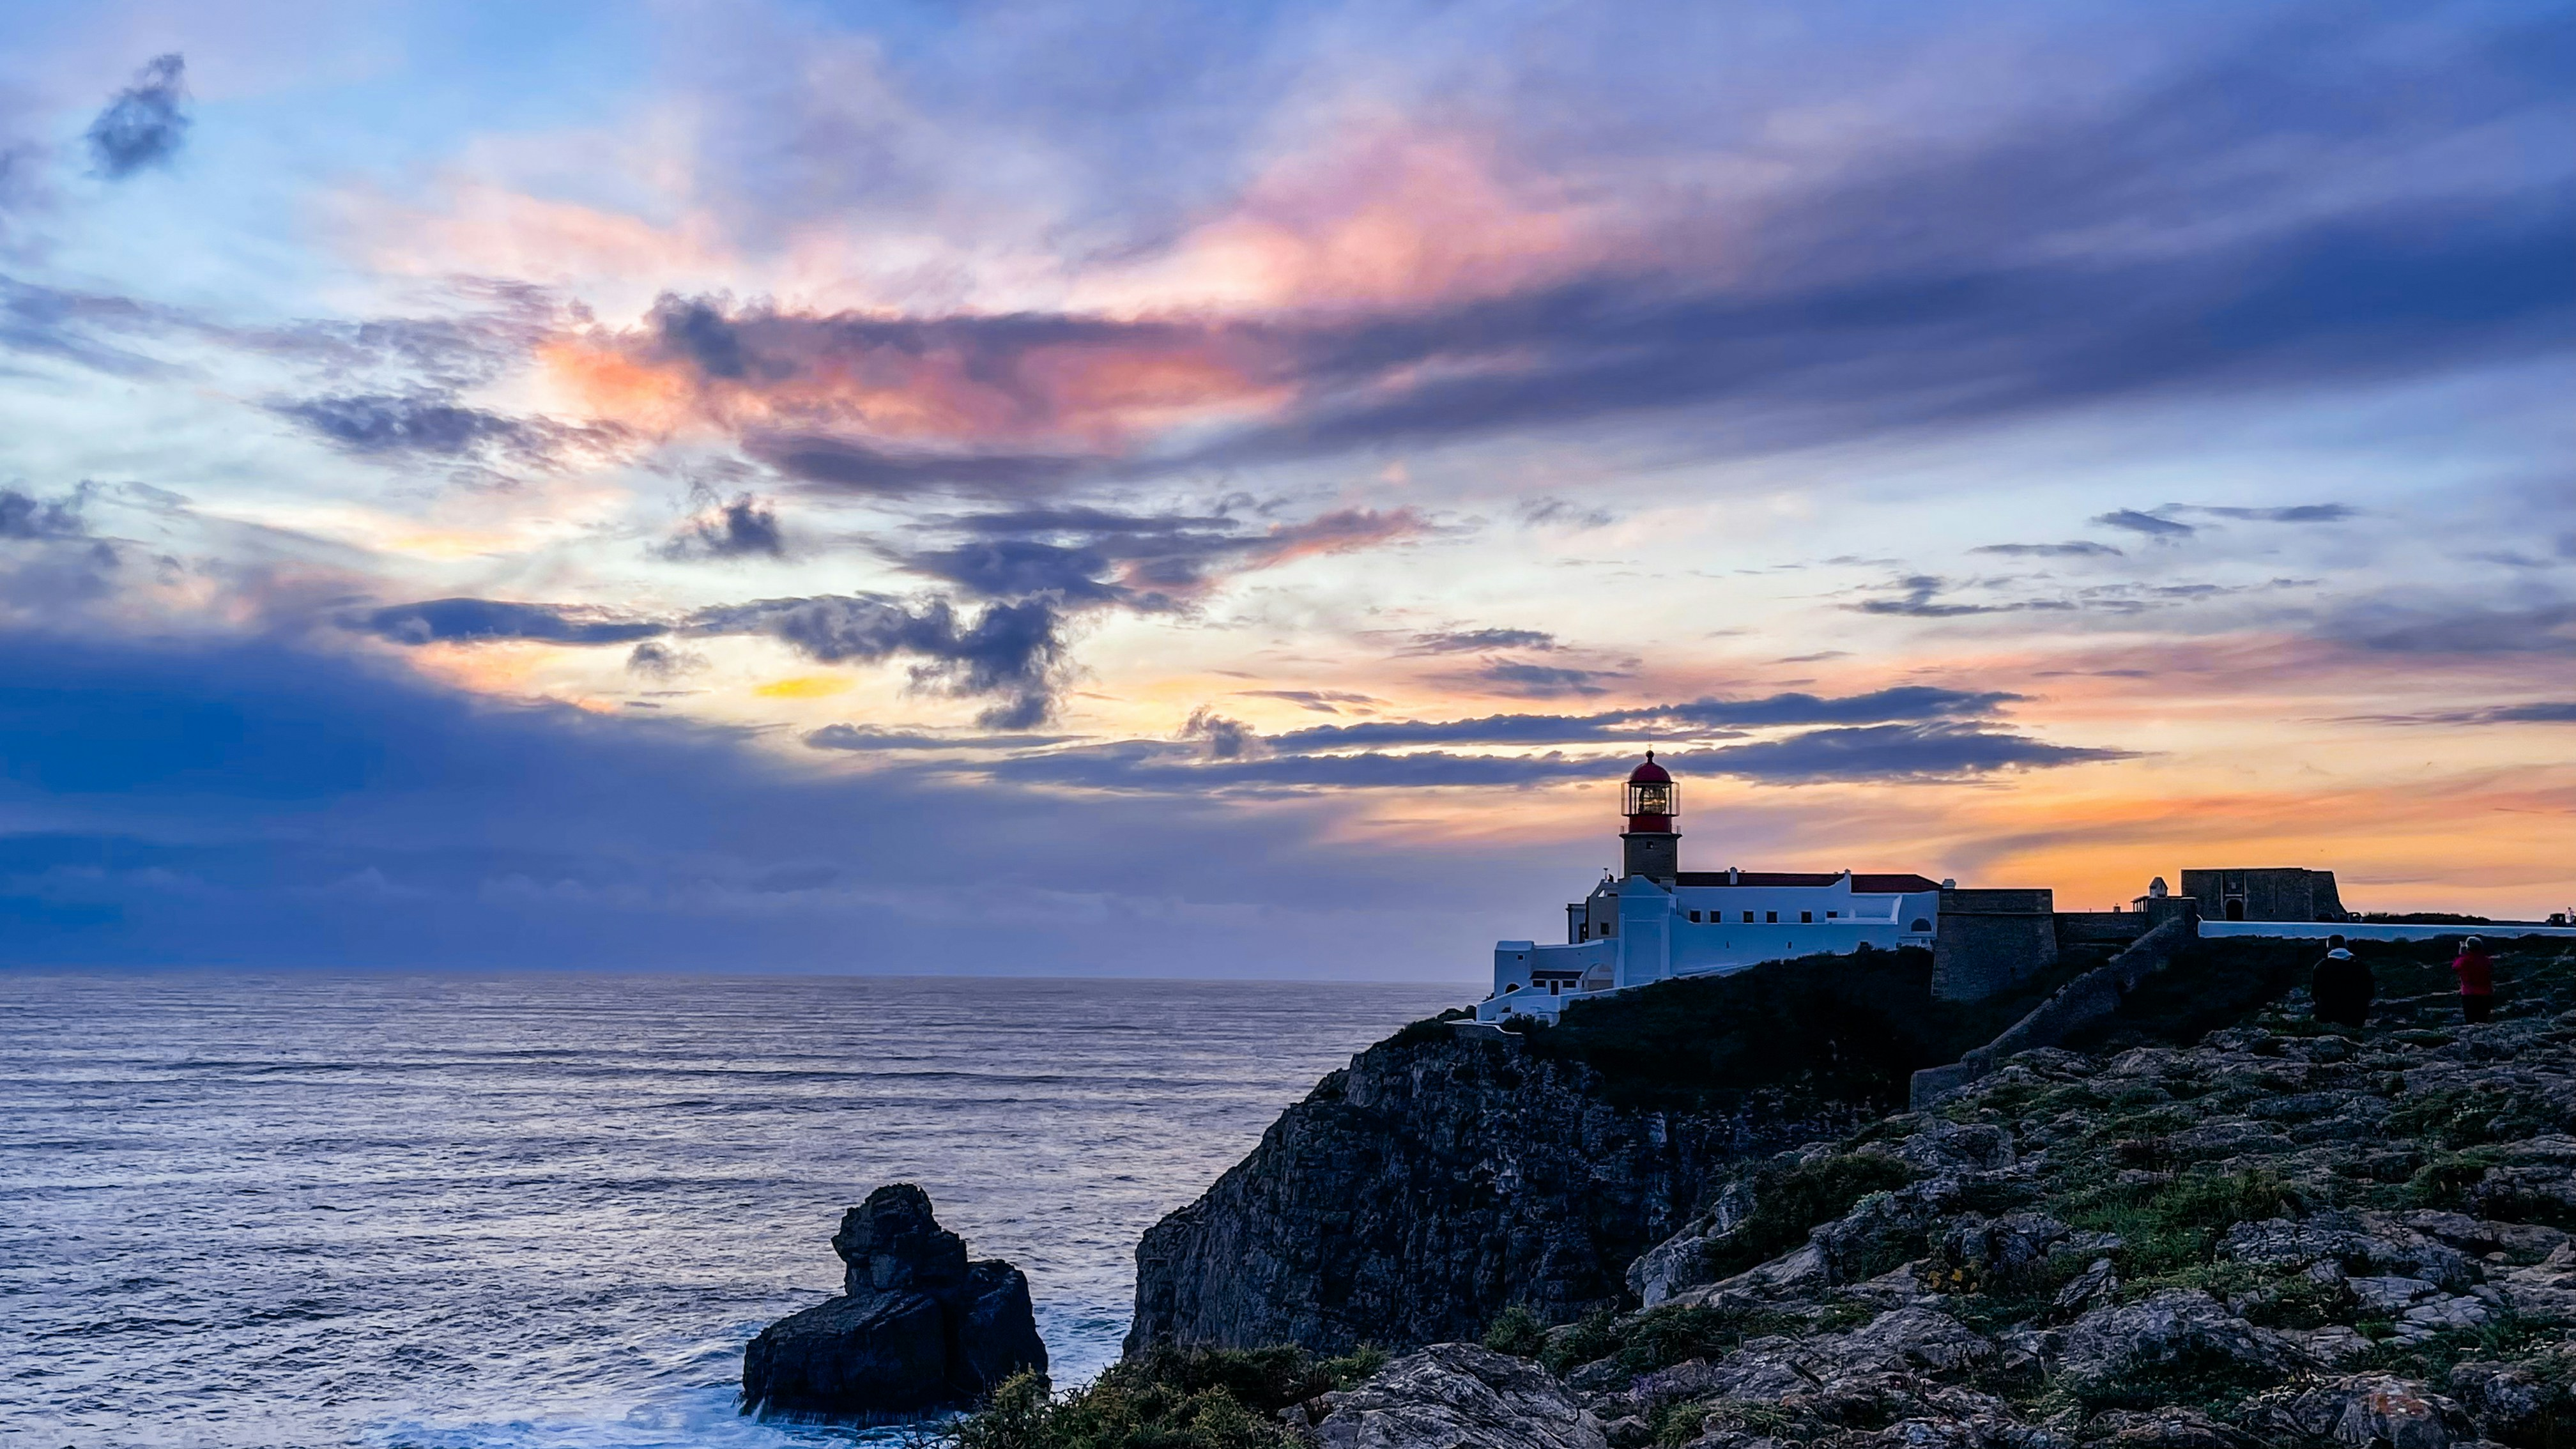
\includegraphics[width=0.9\linewidth]{pngs/image3.png}
  \caption{\textbf{Qualitative comparison.} Replace this placeholder with representative outputs, examples, or visual comparisons.}
  \label{fig:qualitative_results}
\end{figure*}

\subsection{Experimental Setup}

Describe the benchmark protocol, baselines, metrics, and statistical testing procedure.
Make clear which results are produced by the proposed method and which are reproduced from prior work.

\subsection{Main Results}

Present the primary quantitative results.
Use tables for numeric comparisons and figures for trends or qualitative behavior.
Discuss the result in terms of the claims made in the introduction.

\subsection{Ablation Study}

Isolate important design choices and report their effect.
Each ablation should answer a specific question about the method.

\subsection{Limitations}

Describe known limitations, failure cases, and conditions under which the method should not be used.
This improves the usefulness and credibility of the final paper.

\section{Applications}

Describe how the proposed method can be used in realistic workflows.
This section is optional, but it is useful when the contribution has downstream value beyond benchmark scores.

\subsection{Application Scenario One}

\begin{figure}[t]
    \centering
    \includegraphics[width=0.95\linewidth]{pngs/image4.png}
    \caption{\textbf{Application example.} Replace this placeholder with an example showing how the method is used in a downstream scenario.}
    \label{fig:application_example}
\end{figure}

Explain the task, user workflow, integration point, and expected benefit.
Refer to Figure~\ref{fig:application_example} when the application is shown visually.

\subsection{Application Scenario Two}

Describe a second use case or deployment setting.
When possible, connect the application back to measurable properties reported in Section~\ref{sec:evaluation}.

\section{Conclusion}

Summarize the paper's problem, method, and main findings in one compact paragraph.
Avoid introducing new technical details in the conclusion.

Then discuss the broader implication of the work, its limitations, and future directions.
This is a good place to mention planned extensions, open questions, or responsible deployment considerations.

\newpage


\clearpage

\bibliographystyle{plainnat}
\bibliography{main}

\clearpage

\beginappendix
\section{Additional Details}
\label{sec:appendix_details}

Use the appendix for material that supports the paper but would interrupt the main narrative.
Typical appendix content includes extended implementation details, additional experiments, annotation instructions, proofs, extra qualitative examples, and dataset documentation.

\subsection{Reproducibility Checklist}

\begin{itemize}
    \item List software dependencies and versions.
    \item Specify hardware used for training and evaluation.
    \item Document random seeds and evaluation protocols.
    \item Provide links or instructions for code, models, and data when they are released.
\end{itemize}

\subsection{Additional Results}

Add supplementary tables, plots, and qualitative examples here.


\end{document}
